\documentclass[paper=a4, fontsize=10pt]{article} % A4 paper and 11pt font size
\usepackage[lmargin=1in]{geometry}
\usepackage{graphicx,float,subfig}
\usepackage[english]{babel} % English language/hyphenation
\usepackage{amsmath,amsfonts,amsthm,tensor} % Math packages
\usepackage[shortlabels]{enumitem} 
\usepackage{sectsty} % Allows customizing section commands



\allsectionsfont{\centering \normalfont\scshape} % Make all sections centered, the default font and small caps

\numberwithin{equation}{section} % Number equations within sections
\numberwithin{figure}{section} % Number figures within sections 
\numberwithin{table}{section} % Number tables within sections 
\setlength\parindent{0pt} % Removes all indentation from paragraphs 

\newcommand{\horrule}[1]{\rule{\linewidth}{#1}} % Create horizontal rule command with 1 argument of height

\title{	
\normalfont \normalsize 
\horrule{.5pt}\\ % horizontal rule
\Large Empirically Leveraging the TCFT\\ 
\horrule{1pt}\\ % horizontal rule
}
\author{}
\date{\normalsize}%\today}



\def\ket#1{\left\vert #1 \right\rangle}
\def\bra#1{\left\langle #1 \right\vert}
\def\ip#1#2{\left\langle #1 \vert #2 \right\rangle}
\def\opex#1#2#3{\left\langle#1\left\vert#2\right\vert#3\right\rangle}
\def\deriv#1 #2{\frac{\text{d}}{\text{d}#2} #1}
\def\fderiv#1#2{\frac{\dd#1}{\dd#2}}
\def\pderiv#1#2{\frac{\partial}{\partial #2} #1}
\def\npderiv#1 #2 #3{\frac{\partial^#1}{\partial #3^#1} #2}
\def\fpderiv#1 #2{\frac{\partial #1}{\partial #2} }
\def\fnpderiv#1 #2 #3{\frac{\partial^#1 #2}{\partial #3^#1}}
\def\fnderiv#1 #2 #3{\frac{\dd^#1 #2}{\dd #3^#1}}
\def\B#1{\textbf{#1}}
\def\cross {\times}
\def\tbf #1{\textbf{#1} }
\def\det {\text{Det}}
\def\comm#1,#2.{\left[ #1,#2\right]}
\def\tr {\text{Tr}}
\def\dd{\text{d}}
\def\at#1{\Big{|}_{#1}}
\def\avg#1{\langle #1 \rangle}
\def \x {\mathbf{x} }
\def\X {\mathbf{X} }
\def\kB {k_B}


\graphicspath{{img/}}
\begin{document} 

\maketitle % Print the title
\section{notation}

\subsection{process}
A `process' $P(\x) \equiv Pr(X=\x|\Lambda=\lambda)$ will be defined as a probability distribution over the set of system trajectories $\x \in X$, conditioned on the system being exposed to the control protocol $\lambda = \lambda(t)$. Similarly, the conditional process $P(\x|a) \equiv Pr(X=\x|X_0=a, \Lambda=\lambda)$ is the probability that the system undergoes trajectory $\x$ conditioned on both starting in state $a$ at time $t=0$ and being exposed to the control protocol $\lambda$. A final useful piece of notation is $p_t(a) \equiv Pr(X_t=a |\Lambda=\lambda)$; combining these yields the following equality $P(\x|a)p_0(a) = P(\x)$ (which would be a bit ponderous to write without the shorthand). 

The reverse protocol associated with $P$ will be denoted as $R(\x) \equiv Pr(X=\x^\dagger|\Lambda=\lambda^{\dagger})$. $R(\x)$ gives the probability that the same system will undergo the trajectory $\x^\dagger$ provided that it is exposed to the reverse control protocol $\lambda^{\dagger}= \lambda(\tau-t)$; similarly $R(\x|a) \equiv Pr(X=\x^\dagger|X_0=a^*, \Lambda=\lambda^\dagger)$ can be defined as well as $r_t(a) \equiv Pr(X_t=a^* |\Lambda=\lambda^\dagger)$. For every trajectory $\x$ of the system of interest, which is defined by a set of values in the phase space of the system ($\x = (x_0 ... x_\tau)$ for discrete time and $\x= x(t)$ for continuous time), we can define also a reversed trajectory $\x^{\dagger} = (x_\tau^*, ... x_0^*)$. The $*$ indicates sending any time odd quantity to its negative value, spin for example. This becomes relevant for the the phase space coordinates of the system, because they contain canonical momentum variables which do change sings under the time reversal conjugation. 

\subsection{Trajectory Classes}
$C$ is defined by a function $c(\x)$ that takes a trajectory to a boolean: $c : \X \to  \mathbb{B}$. Of all possible trajectories $\x \in \X$, $C$ is the set of trajectories for which $c(\x)$ is True. In standard mathematical notation, $C: \{\x \in \X | c(\x)\}$. This notation allows us to define the reverse class $C^{\dagger}$ clearly, $C^{\dagger} : \{\x \in \X | c(\x^{\dagger}) \}$. Note that the $\x^\dagger$ `reverse trajectories' come from the same space as the `forward trajectories'. The dagger operator acting on a trajectory means conjugate time reversal, if we think of trajectories over a time $\tau$ as being composed of a bunch of instantaneous position and momentum coordinates $\x(t) = (x_t, v_t) \forall t \in [0,\tau]$ then $\x^{\dagger}(t) = (x_{\tau-t}, -v_{\tau-t})$. 

As an example, consider a class of all trajectories with positive initial velocity, and so defined by the function $c(\x) = \left[  v_0 > 0 \right]$. Suggestively, the class can be called  $v_{0+}$. The reverse class $v_{0+}^{\dagger}$ is 
\begin{align}
v_{0+}^{\dagger} : \{ \x \in \X | c(\x^\dagger)\} \\ 
v_{0+}^{\dagger} : \{ \x \in \X | -v_\tau > 0\} \\ 
v_{0+}^{\dagger} : \{ \x \in \X | v_\tau < 0\}
\end{align}
We see that reverse class is the set of trajectories that end with a negative velocity; we might, for example, call it $v_{\tau-}$.

\section{core results to highlight}

\subsection{Proof Sketch}
The integrated TCFT can be derived from the existence of a generalized detailed fluctuation theorem between a trajectory wise quantity $\Omega(\x)$, a process $P(\x)$  and a process conjugate to $\Omega$ called $P^\Omega(\x)$. $P^\Omega(\x)$ is the probability of the same trajectory in the conjugate process, though at this point the form of the conjugacy is left completely general. It is whatever it needs to be to satisfy the equality
\begin{align}\label{eq:GeneralConjugacy}
\frac{ P(\x)}{P^\Omega(\x)} = e^{\Omega(\x)}
\end{align}
Assuming a conjugacy of the form above, deriving a TCFT is very straightforward: simply integrate over some measurable subset of trajectories (There are some details about integration that are important mathematically, but not necessary to understand the shape of the proof. For a rigorous proof, refer to \tbf{cite TCFT}.)
\begin{align}
 \int_C P(\x) e^{-\Omega(\x)} &=  \int_C P^\Omega(\x)\\
 \int_C P(C)P(\x|C) e^{-\Omega(\x)} &= \int_C P^\Omega(\x) 
\end{align}
The second equality comes from the fact that $P(\x)=P(\x,C)$ because the integration is over trajectories in $C$ only. Recognizing that $P(C)$ is independent of the integrand, the final line can be rearranged to read:
\[  \avg{e^{-\Omega}}_{C}= \frac{P^\Omega(C)}{P(C)} \]
This is a very general statement of the TCFT, but under relatively common assumptions it can be easily interpreted alongside other common fluctuation theorems. If the system is coupled to a sufficiently ideal heat bath at inverse temperature $\beta$ and the reverse process has the property that $r_0(x_\tau) = p_\tau(x_\tau)$-- the Crooks detailed fluctuation theorem \tbf{CITE CROOKS} takes the form of equation \ref{eq:GeneralConjugacy} in which $P^\Omega(\x) = R(\x)$, and $\Omega=\Sigma$. Here, $R(\x)$ is as described in the previous section, and $\Sigma$ is the entropy production $\Sigma(\x) \equiv -\beta Q + \ln \frac{p_0(x_0)}{p_\tau(x_\tau)}$. Q is the heat absorbed by the system from the bath, so $-\beta Q$ is the entropy generated in the thermal bath. In this setting, the TCFT becomes:

\[  \avg{e^{-\Sigma}}_{C}= \frac{R(C)}{P(C)} \]


\subsection{Trajectory Class Jarzynski Equality}\label{sec:TCJE}
In the spirit of usual FT methods , we set the initial distribution for $P$ is the equilibrium distribution associated with $\lambda_0$, $\pi_0$ and the initial distribution for $R$ is the equilibrium distribution for associated with $\lambda_\tau$, $\pi_\tau$. Using a first law $\Delta E = Q + W$ for the system, the entropy production breaks into
\begin{align}
\Sigma(\x) &= \beta (W-\Delta E) +  \ln \frac{\pi_0(x_0)}{\pi_\tau(x_\tau) }\\
 &= -\beta (H_S(x_\tau,\lambda_\tau)-H_S(x_0,\lambda_0) - W) + \ln \frac{ Z_\tau e^{-\beta H_S(x_0,\lambda_0)}}{Z_0 e^{\beta H_S(x_\tau,\lambda_\tau})} \\
 &= \beta W + \ln \frac{ Z_\tau}{Z_0} \\
&= \beta( W(\x) -  \Delta F) = W_d
\end{align}
The result is a class conditioned version of the Jarzynski equality estimation of the free energy, containing a correction term compensating for the incomplete integration:
\begin{align}
\label{eq:TCFTJarzynski}
 \avg{e^{-W_d}}_{C}= \frac{R(C)}{P(C)} \\
e^{\beta \Delta F} \avg{ e^{-\beta W}}_C =  \frac{R(C)}{P(C)} \\
\beta  \Delta F = - \ln \avg{ e^{-\beta W}}_C - \ln \frac{P(C)}{R(C)}  
~.
\end{align}
The takeaway is that a fluctuation theorem can estimate the equilibrium free energy in a process where it is not possible to sample all trajectories. The tradeoff when compared to the JE is a need for additional information: the probabilities of the trajectories in both the forward and reverse process. This opens up the ability to avoid regions that might suffer from the existence of very rare but very dominant events, which will be discussed more in section \ref{sec:Corrections}

\subsection{Nonequilibrium Free Energy}

The result in section \ref{sec:TCJE} is actually a special case of a more general results. For a larger class of processes, the trajectory wise entropy generation can be written as $\Sigma(\x) = \beta(W(\x) - \Delta f(\x, \rho_\tau, \rho_0)) $ where we have defined a pointwise free energy $f(x,\rho) = E(x) + \beta^{-1} \ln \rho(x)$ and a  trajectory wise free energy difference $\Delta f(\x, \rho_\tau, \rho_0) = f(x_\tau,\rho_\tau) - f(x_0,\rho_0) =  \Delta E(\x) + \beta^{-1} \ln \frac{\rho_\tau(x_\tau)}{\rho_0(x_0)}$. These free energies are often referred to as 'nonequilibrium free energy' because they define a free energy over arbitrary distributions. In the case above, the normal equilibrium free energy falls out because $F_\lambda = -\beta^{-1} \ln Z_\lambda = f(x, \pi_\lambda)$. However, we can also ask questions about the nonequilibrium free energy difference proper. From this perspective, as long as we choose a class for which all trajectories have the same nonequilibrium free energy difference $\Delta f(\x, \rho_f, \rho_0) = \Delta f_c \enskip\forall\enskip \x \in C$ the TCFT result from equation \ref{eq:TCFTJarzynski} will apply:

\[ \beta  \Delta f_c = - \ln \avg{ e^{-\beta W}}_C - \ln \frac{P(C)}{R(C)}  \]

An interesting extension assumes that we partition all trajectories in classes defined by their $\Delta f$, and then average over all classes:
\begin{align}
 \beta \avg{ \Delta f} &=  \beta \sum_c P(C) \Delta f_C \\
 &= -\sum P(C) \ln \avg{e^{-\beta W}}_C + \sum P(C) \ln \frac{P(C)}{R(C)} \\
&= - \ln \avg{e^{-\beta W}} + \sum P(C) \ln \frac{P(C)}{R(C)} \\
& = \beta \Delta F+ \sum P(C) \ln \frac{P(C)}{R(C)}
\end{align}
$P(C)$ and $R(C)$ are two distributions over the set of trajectory classes and so the last term can be written as $D_{KL}(P||R)$. Thus the equilibrium free energies can be written in terms of a weighted average over all possible non-equilibrum free energies and coarse-grained statistics on the partitioning. While it isn't, at this point, clear how to access $f$ experimentally in a general way, it can at least be argued that this tells us the average $\avg{\Delta f}$ is bounded from below by the change in equilibrium free energy through the positivity of the $D_{KL}$. \tbf{Not really sure if/how to use this}

\subsection{Metastable Free Energy}
A notable set of processes/classes that allow for easy partitioning into classes of constant and physically interpretable $\Delta f$'s are processes that begin and end in metastable distributions. A metastable distribution means that the state space can be separated into metastable regions inside of which the distribution appears equilibrium-- though it need not be globally in equilibrium. This is typical in a `computational' physical setting-- which requires the coexistence of multiple distinguishable, long lasting, informational states $m$. Memory states $m$ are defined by a coarse graining on the space of $X$ by a partitioning the full state space into subsets $\{X_m\}$. A metastable distribution can be described by a set of  $\rho^m (x) = w^m \pi^m (x)$ where $\sum_m w^m =1$. The $\pi^m(x) = \frac{1}{Z^m} e^{-\beta E(x)} $ are the local equilibrium distributions and are unique for a given process with $Z = \sum_m Z_m$. $w_i$, the relative weights of the regions, are not unique; they are only subject to the normalization constraint. Note that these $Z^m$ define `local free energies' $F^m = -\beta^{-1} \ln Z^m$. The probability of a point in phase space, $x$, in a metastable distribution is $\rho(x) = \delta_{xm} \rho^m(x)$ (here $\delta_{xm}$ is the Iverson bracket $\delta_{xm} = \left[ x \in\{X_m\} \right]$). 

If a process begins in metastable distribution $\rho_{\lambda_0}(x, \{w\})$ and ends in a metastable distribution $\rho_{\lambda_\tau}(x, \{u\})$, the nonequilibrium free energy difference for a trajectory that starts in metastable region $i$ and ends in metastable region $j$ is:

\begin{align}
 \Delta f_{ij} &= E(x_\tau) + \beta^{-1} \ln u^j \pi^{j}(x_\tau) -E(x_0) - \beta^{-1} \ln w^i \pi^i(x_0) \\
  &=  \beta^{-1} \ln\frac{u^j}{Z^j}  - \beta^{-1} \ln \frac{w^i}{Z^i} 
\end{align}
Importantly, the trajectory dependence is gone so this is a case of a class of constant free energy difference.
\begin{align}
\beta \Delta f_{ij} &=  \ln \frac{u^j}{w^i}  +  \beta \ln \frac{Z^i}{Z^j} \\
&= \beta \Delta F^{ij} + \ln \frac{u^j}{w^i}
\end{align}
Here, the explicit definition of $\Delta F$ is $\Delta F_{ij} = F^j_{\lambda_\tau} - F^i_{\lambda_0}$, a difference of `local free energies' for the memory states $i$ and $j$ for any process with the given control protocol. The quantity $\Delta f_{ij}$ we call the difference in metastble free energy. Metastable free energy being defined as $f^m \equiv F^m + \beta^{-1} \ln w^m$. These metastable free energies are a special case of the nonequilibrium free energy-- which means it tells you the minimum average work it takes to drive an ensemble of particles in the initial well with the given initial weight to the second well with the second weight. Plugging this case into equation \ref{eq:TCFTJarzynski} yields:
\begin{align}\label{LocalFreeEnergy}
\beta \Delta F_{ij} =  -\ln \avg{e^{-\beta W }}_{ij}- \ln \frac{P(C_{ij})}{R(C_{ij})} - \ln \frac{u^j}{w^i} 
~. 
\end{align}

An important thing to note here is that while $R(C_{ij})$ means the probability of $C_{ij}^{\dagger}$ in the reverse process,t the initial distribution of the reverse process is undetermined. Determining this is absolutely crucial and different choices will give different results. One such example is setting the initial weights of the forward and reverse process such that $ \ln \frac{P(C_{ij})}{R(C_{ij})} + \ln \frac{u^j}{w^i} =0 $. In this case, averaging over the local free energies for all possible combinations of memory states will the equilibrium free energy change of the computation. This approach might be be useful to leverage the accuracy of several careful experiments that start in particular memory states rather than attempting to find the entire work distribution all at once.

\section{Examples/Sims}

\subsection{Correcting Experimental Errors with the TCFT}\label{sec:Corrections}

In a typical experiment to estimate free energy using the nonequilibrium work distribution, one might perform the following:
\begin{enumerate}
\item initialize a system in equilibrium
\item drive the system out of equilibrium, measuring the work $W$ needed to do so
\item repeat the above using the same driving protocol $N$ times
\item use statistics to find $ \bar{JE}  = \frac{1}{N} \sum_{i=0}^N e^{-\beta W_i} \approx \avg{e^{-\beta W}}$ and its variance $s^2_{JE}$
\item use $\bar{JE}$ and $s^2_{JE}$ as estimators for the free energy and the variance of the estimate using the JE
~.
\end{enumerate}

In \tbf{CITE Jarz Rare Event}, some of the pitfalls of this method are discussed. In this section, we compare the baseline approach of free energy estimation outlined above to an augmented method that requires also an experiment of the reverse process and uses the TCFT (equation \ref{eq:TCFTJarzynski}):

\begin{align}
\beta \Delta F = -\ln \avg{e^{-\beta W}} - \ln \frac{P(C)}{R(C)}
~,
\end{align}
to estimate the free energy. Rather than analyze the cases analytically, we will turn to numerics here. A simple protocol will be outlined, and then a large ensemble of realizations will be simulated.

Since the exact free energy is known, it will be a simple matter to estimate it through different methods and compare the methods.
Before talking specifically about an example system, we briefly touch on error estimation in these systems.  In a general sense, when using the TCFT, there are three sources of error instead of just one because $P(C)$ and $R(C)$ need to be estimated as well. However, since these are sample proportions rather than sample means-- their error scaling is straightforward. Using the formula $\sigma^2_{\ln x+\ln y} = \left(\frac{\sigma_x}{\avg{x}}\right)^2 + \left(\frac{\sigma_y}{\avg{y}}\right)^2$ for two uncorrelated variables, we assume that
\begin{align} \label{ref:VarianceCalc}
\sigma^2_{\Delta F} =\left(\frac{\sigma^2_{JE}}{\bar{JE}}\right)^2 + \left(\frac{\sigma^2_P}{\hat{P}(C)}\right)^2 + \left(\frac{\sigma^2_R}{\hat{R}(C)}\right)^2
\end{align}
where the variances for each variable are calculated using the standard formulas for sample means and standard deviations for variables that satisfy the central limit theorem. Using the full JE is akin to choosing the class of all trajectories. The benefit is that there is no uncertainty in $P(C)$ or $R(C)$ as they both equal 1 with certainty; the downside is that you must take an average over all possible trajectories-- which includes the exponentially rare, but dominant events.

\subsection{The Untilt Process}
In order to provide a simple example of a metastable process, we investigate an `untilt' control protocol. Using 1D Langevin dynamics, as described in section, we set the potential energy to have only two potential energy minima located at $x = \pm x_0$. At $t=0$, the well corresponding to the memory state $m_x=1(m_x=0)$ (our convention sets this memory state to be defined by the region $x>0(x<0)$) will have a depth of $U_1$($U_0$). Initially, $U_1 > U_0$ which means that the equilibrium distribution at this time favors being in the right well.  As time progresses from $t=0$ to $t=\tau$, the right well is raised linearly with time until $U_1=U_0$ (see figure for the energy landscapes and equilibrium distributions \ref{fig:Untilt}). This is done on a timescale that is faster than the time it would take for the wells to equilibrate between each other, but slow enough that the local distributions conditioned on being in each well are not perturbed very far away from equilibrium. The reverse simulation, following section \ref{sec:TCJE} will begin in the equilibrium distribution associated with the $U_1=U_0$ energy landscape-- and then follow the reverse protocol of lowering the energy of the right well.

\begin{figure}[H]
\centering
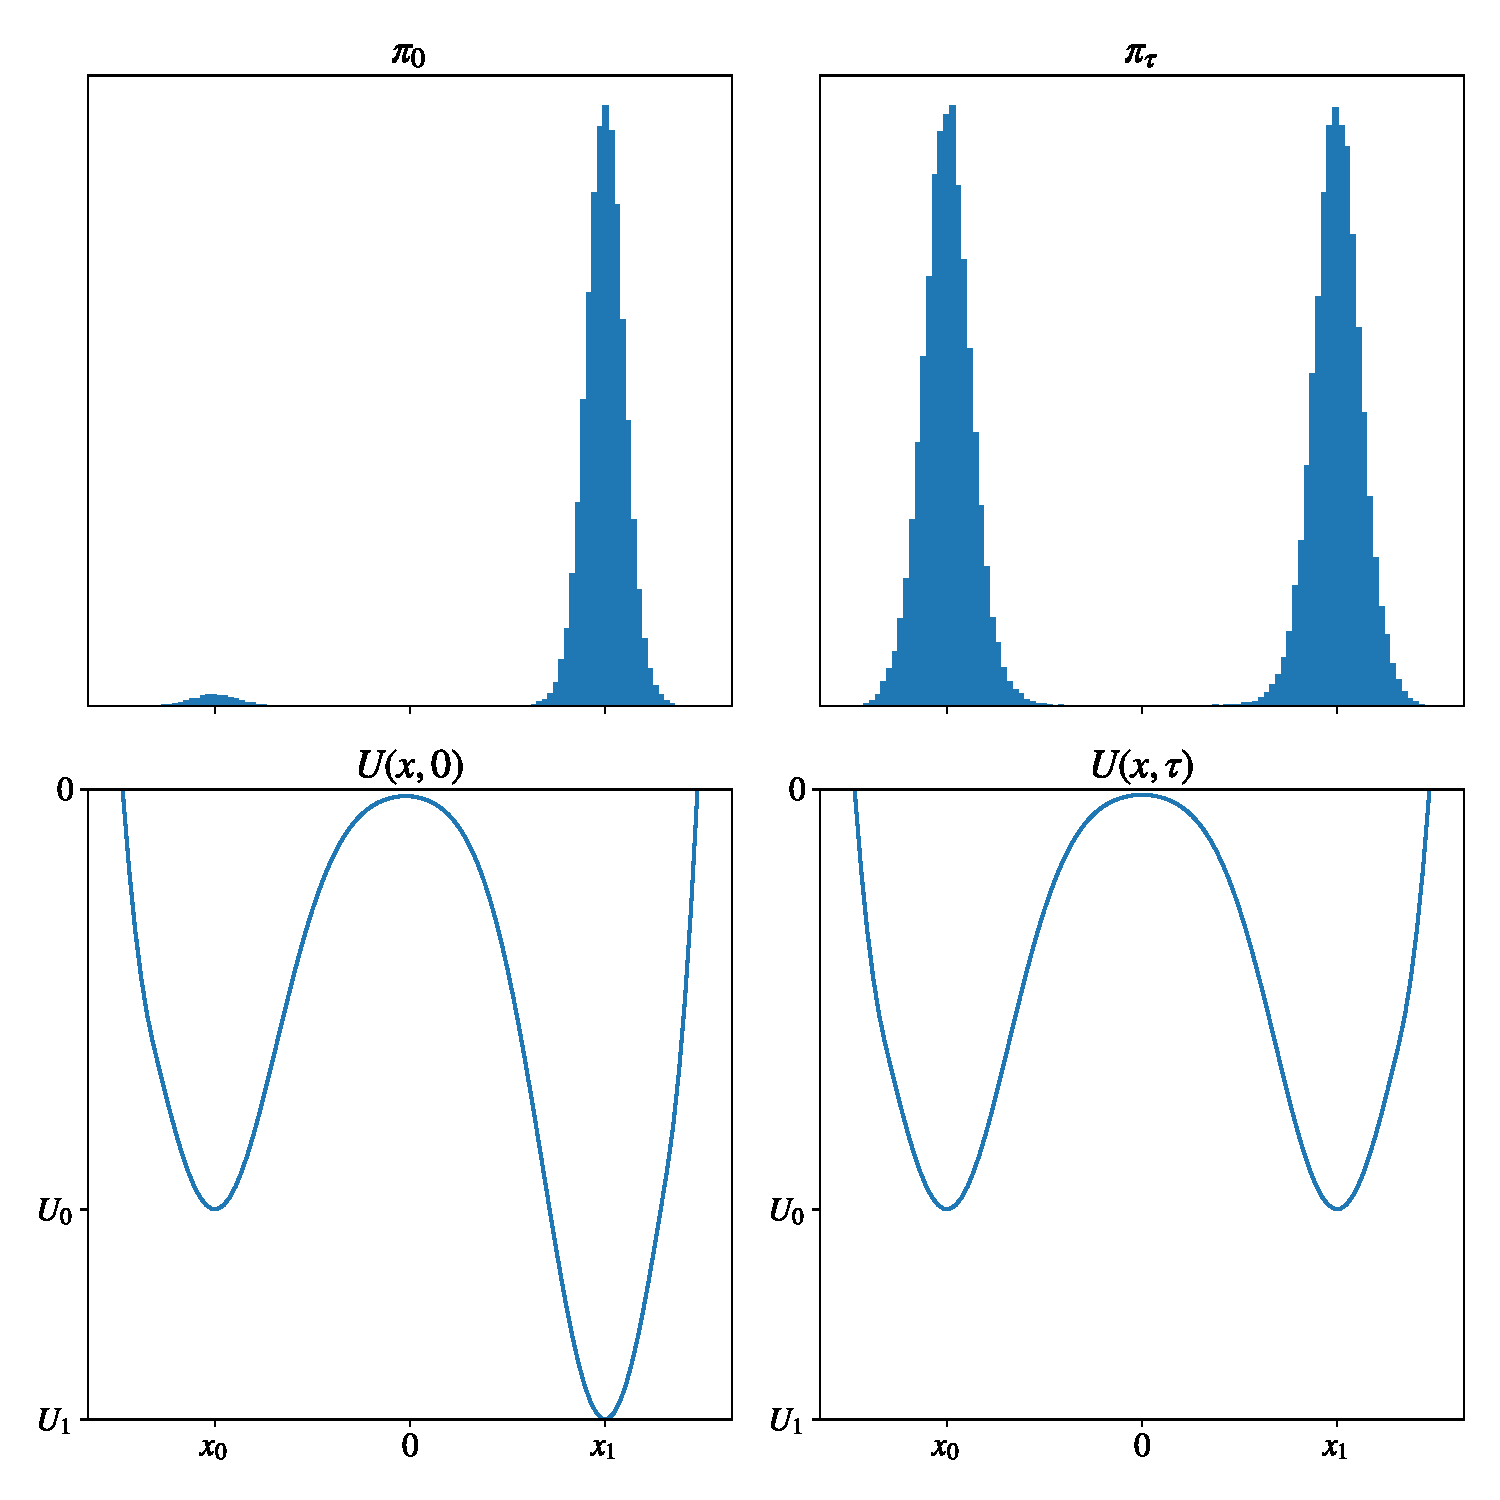
\includegraphics[width=.6\columnwidth, trim=0 0 0 0, clip]{untilt.pdf}
\caption{The initial and final equilibrium distributions and potential energy profiles for the untilt process; under the exchange of $\tau \leftrightarrow 0$, the same but for the reverse untilt process.}
\label{fig:Untilt}
\end{figure}


Our first numerical experiment will go as follows:
\begin{enumerate}
\item Sample a large ensemble of initial conditions from the equilibrium distribution for both the forward and reverse processes.
\item Simulate the the system being driven out of equilibrium in both processes, and measure the work $W$ needed to do so for each trajectory. 
\item Take a sample out of of a specific size $n$ from the forward process trajectories
\item Use the samples statistics to estimate the free energy change during the protocol using the JE and the forward process only, as described above
\item Take a sample out of of a specific size $n$ from the reverse process trajectories
\item Use the samples' statistics to estimate the free energy change during the protocol using the TCFT (equation \ref{eq:TCFTJarzynski}) under a suite of different trajectory classes
\item Repeat steps 3-5 with another value of $n$ to observe how the different estimates converge
\end{enumerate}

The process above was carried out with an ensemble of 500,000 trajectories and $n=$1,000, 4,000, 20,000, and 100,000. Figure \ref{fig:VarScaling} displays the results. With the intent of showing how the various possible trajectory classes behave in a stripped down example, a suite of different trajectory classes are investigated:
\begin{enumerate}
\item The most basic trajectory class `jarz' is the set of all trajectories. This trajectory class is simply using the traditional JE, and gains nothing from reverse process. \tbf{revisit these descriptions. use less classes and make sure that the expectations actually met up with the simulation}
\item $v_{i+}$ trajectories for which the initial velocity is positive, and its complement $v_{i-}$ for which initial velocities are negative. The conjugate classes for these two are $v^\dagger_{i+} = v_{f-}$ and $v^{\dagger}_{i-}=v_{f+}$. Because both processes begin and end in equilibrium, these classes are not expected to be advantageous-- there is no coupling between position and velocity in the equilibrium distribution so we would expect these two classes to have the same attributes as the entire trajectory set-- but with approximately half the sample size. These classes are expected to be outperformed by the traditional JE in every way. They should be similarly unbiased as estimators, but there is nothing to be gained from using this class instead of the full set of outcomes
\item $x_{i<}$ and its complement $x_{i>}$ (and their conjugate classes $x_{f<}$ and $x_{f>}$) represent trajectories that start close(far) from the minimal of their local potential well. The idea of these classes is to separate initial conditions that are typical of the equilibrium distribution and those that represent large fluctuations in energy. In the figures that follow, the threshold was set so that the typical class contained $~68\%$ of initial conditions. It is not clear which of these should provide better estimates. On the one hand, one might think that the larger energy fluctuations explore more of the state space and so can provide more information about the energy landscape. On the other hand, the sample size is smaller and the proportions will be far from the case of $\hat{p}=.5$, for which the variance is the smallest.
\item $x_{max<}$ and its complement $x_{max>}$ have the same conditions as the previous two classes, but applied over the entire trajectory rather than just the initial point. Rather than separating into trajectories that start out as large fluctuations or not, the separation is into trajectories that don't experience any unusual fluctuation and those that do (note that the conjugate classes for these two are the same as the forward classes.) Keeping the same threshold as above yielded approximately $20\%$ of trajectories in the in first and $80\%$ in the second. Thus, the issue of the larger fluctuations having a small probability is ameliorated. Therefore, relative to the analogous classes above we can expect each to perform worse and better respectively.
\item $m_{i \neq f}$: this trajectory class is the set of `transitional' trajectories that end in a different memory state than they start in. The conjugate class is the same as the original class since the class contains two event $m_i=0, m_f=1$ and $m_i=1, m_f=0$ that map to each other under $C^{\dagger}$ which swaps the $i$ and $f$ but not the memory state (which is a coarse graining of a time symmetric variable.) Because of the protocol design, the probability of such a trajectory will be very low in the forward process. This should make it nearly impossible to get good statistics. This class implies two complementary classes $0$ and $1$, which are the two classes that stay in the well they begin in for the entire protocol.
\item The final trajectory class, $W_{>}$ contains trajectories that have a work cost higher than a particular threshold, in this case $W > .8 \kB T$ which makes up about $96\%$ of simulated trials. Its conjugate class is the set of trajectories that cost work less than the negative of the threshold $W< -.8 \kB T$ and makes up about $50\%$ of the trajectories in the reverse process. This class intentionally neglects the exponentially damped work outcomes that have very negative values, in an attempt to avoid the problems of rare event dominance. Crucially, even though these events dominate the average-- the TCFT should allow an `un-biasing' of the estimate given proper statistics on the reverse protocol.
\end{enumerate}

\begin{figure}
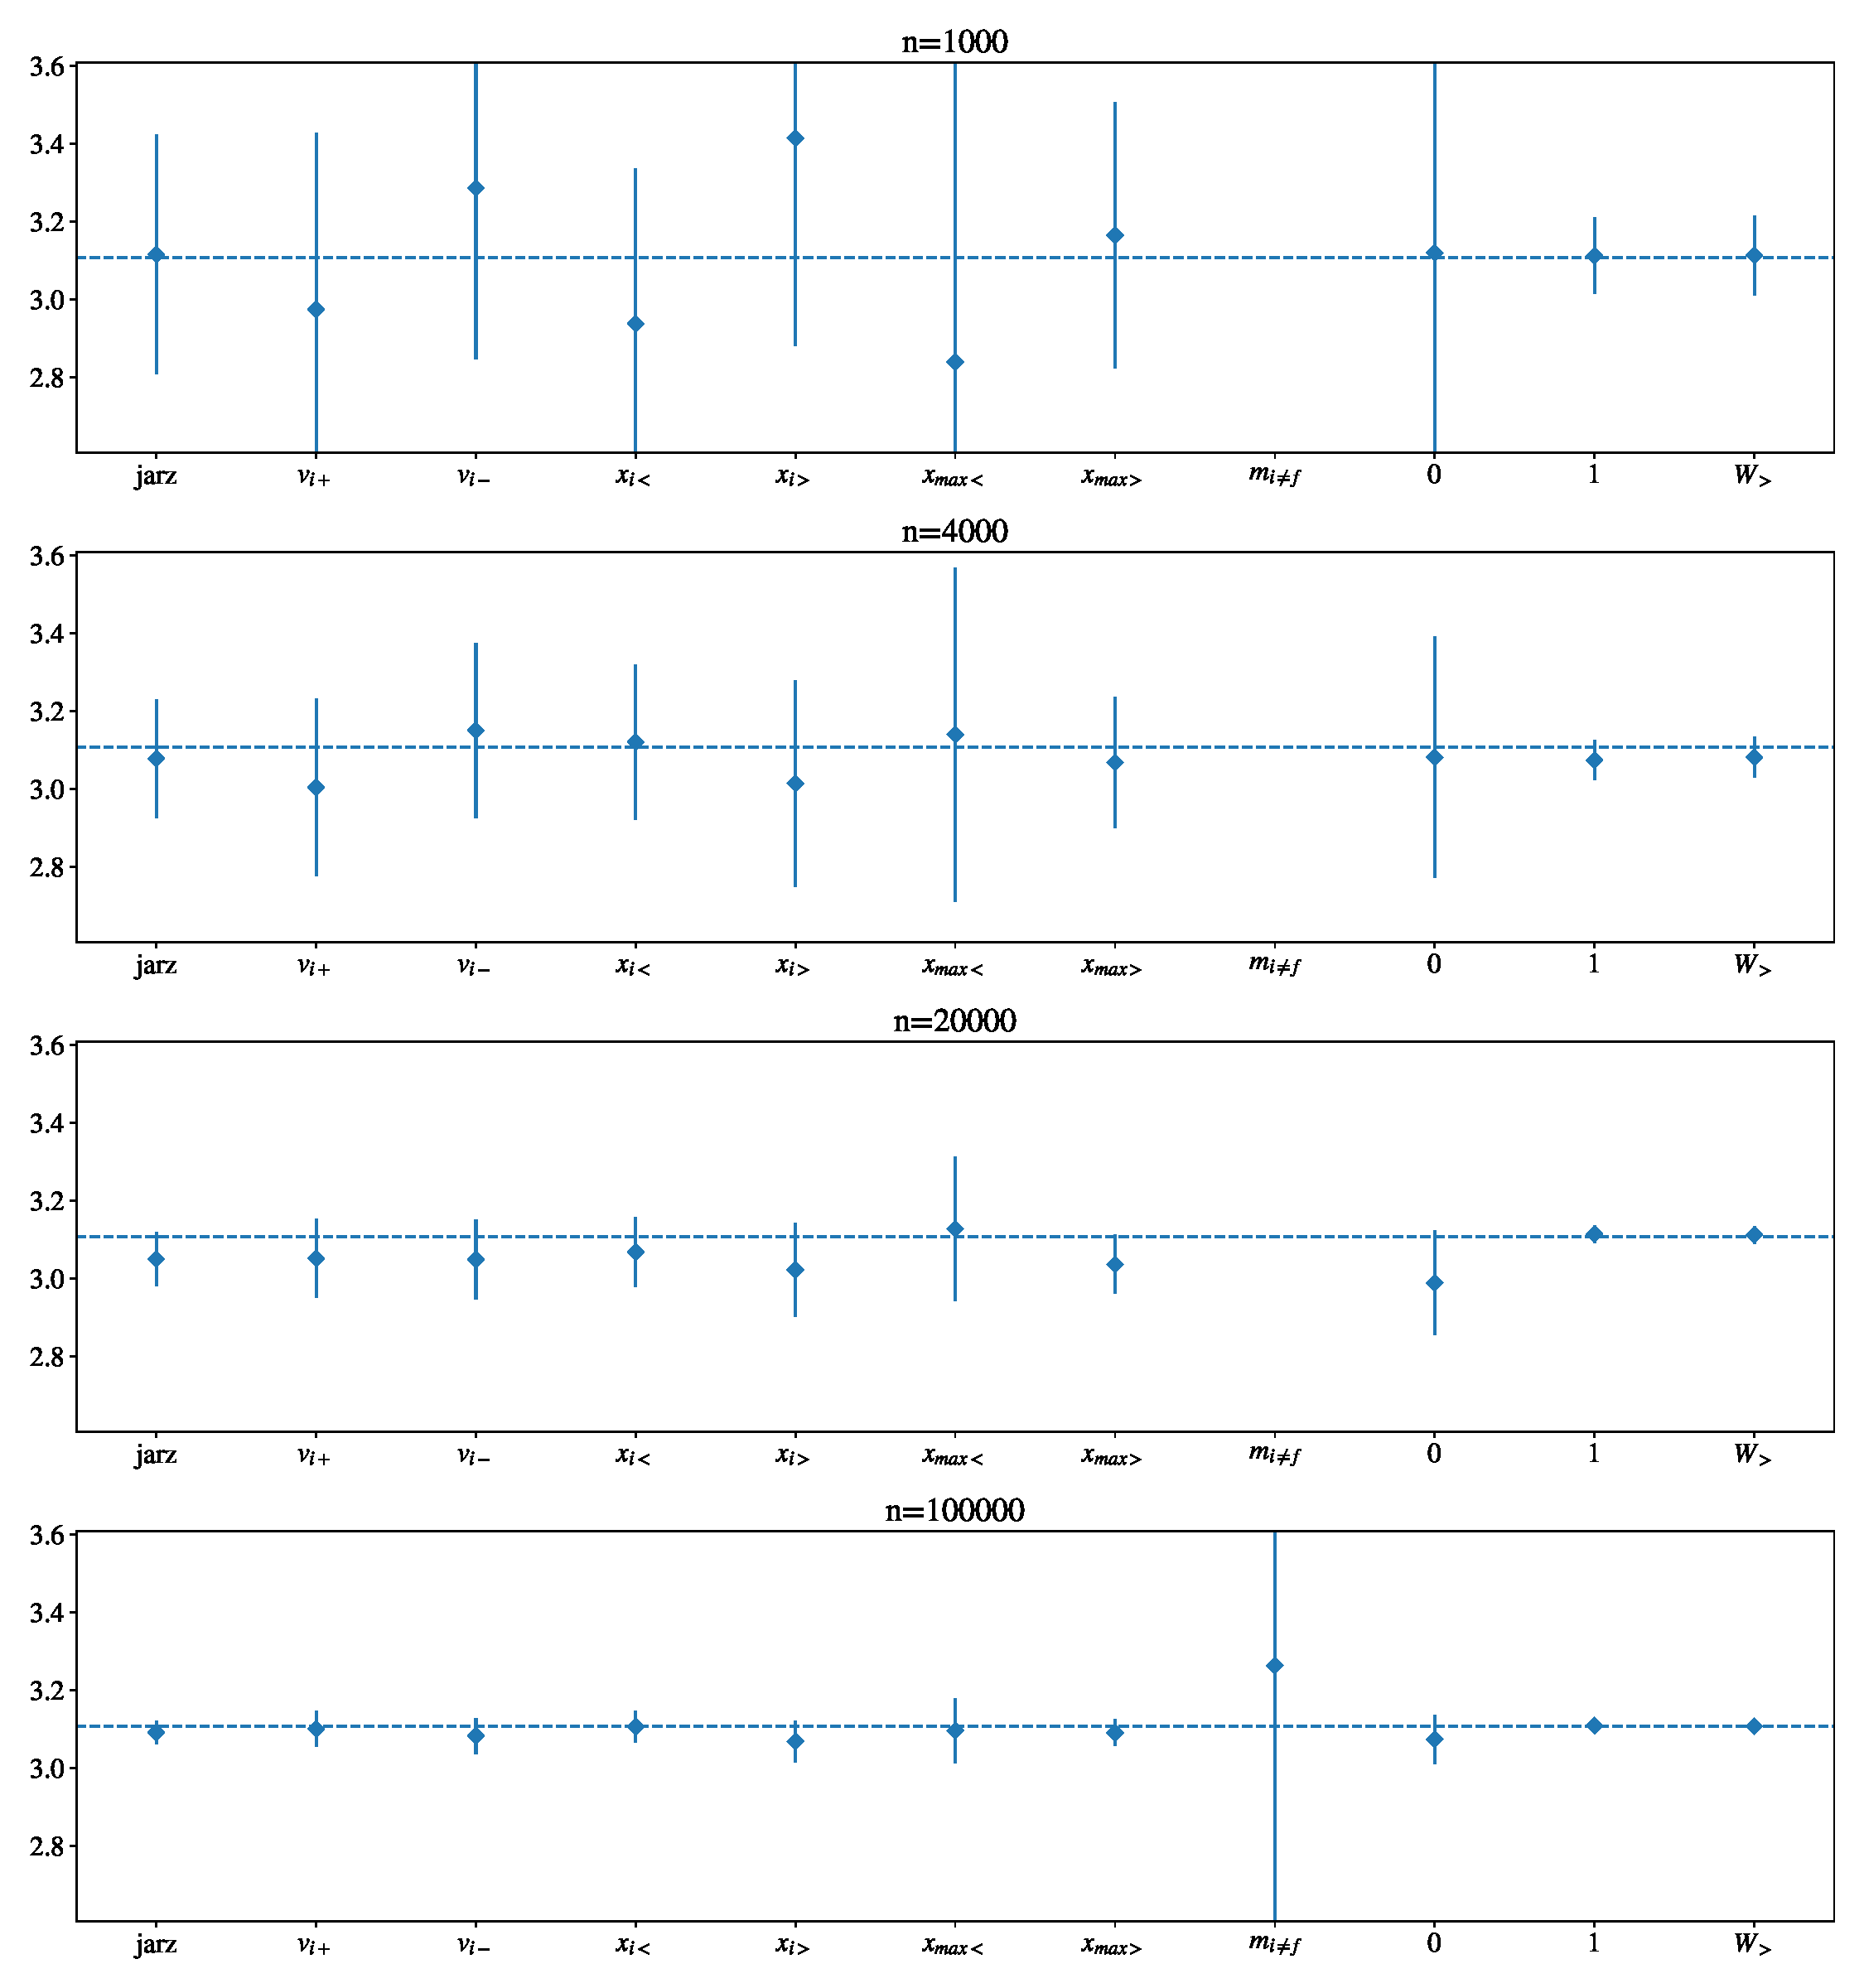
\includegraphics[width=\columnwidth, trim=0 0 0 0, clip]{Variance_Scaling.pdf}
\caption{The results of applying the TCFT to the suite of trajectory classes described in the text. We can see that each class behaves in accordance with the expected behavior. Not also that in every single case, an unbiased estimator is formed, even if the trajectory class in question is very biased. Remarkably, there exist trajectory classes that work better to estimate the free energy than just using all trajectories. The two best trajectories are $1$ and $W_>$, which have high probabilities in the forward process without being especially rare in the reverse process. This allows for the benefit of being able to ignore rare forward process events without offsetting the gain in uncertainty with a high uncertainty in $R(C)$. The transitional class $m_{i\neq f}$ is so rare that the a sample is not likely to even contain a single trajectory in both the forward and reverse processes until $n\approx 100,000$.}
\label{fig:VarScaling}
\end{figure}
To really appreciate the TCFT, it is informative to focus in on a class like the $0$ class. A remarkable feature of the $0$ class, is that it is an incredibly unlikely set. In the forward process, the probability that a trajectory occupies only the $0$ state for the entire protocol is only about $2\%$. However, provided that a good estimate can be made of the class probability in the reverse process ( it is known to be $\approx .5$ from the setup of the untilt process, but it is estimated by the reverse process statistics in plots anyway), a mere $2\%$ of trajectories can form an unbiased estimator of the free energy. This can be seen in figure \ref{fig:ErrorCorrection} which shows a histogram of 100 different attempts at estimating the free energy using only $1000$ trajectories each time. While using all trajectories will provide a lower variance between different attempts, the fact that such a highly biased and unlikely trajectory class can provide an unbiased estimate is staggering. While one might expect the TCFT to do little for the $1$ class, which already makes up close to $98\%$ of all trajectories, figure \ref{fig:ErrorCorrection} shows the variance when using the TCFT is significantly lower, even though both estimates appear to be unbiased. A counter argument is that the TCFT uses twice as many trajectories to estimate (since information is needed about two different processes), but the reduction in variance is more than what would be expected by using twice as many trajectories in the forward process and ignoring the TCFT. In that case, the error would be expected to shrink by a factor of $\frac{1}{\sqrt{2}} \approx .707$; however, the use of the TCFT shrinks the variance by $\frac{.0907}{.0295} \approx  .325$.

\begin{figure}
\centering
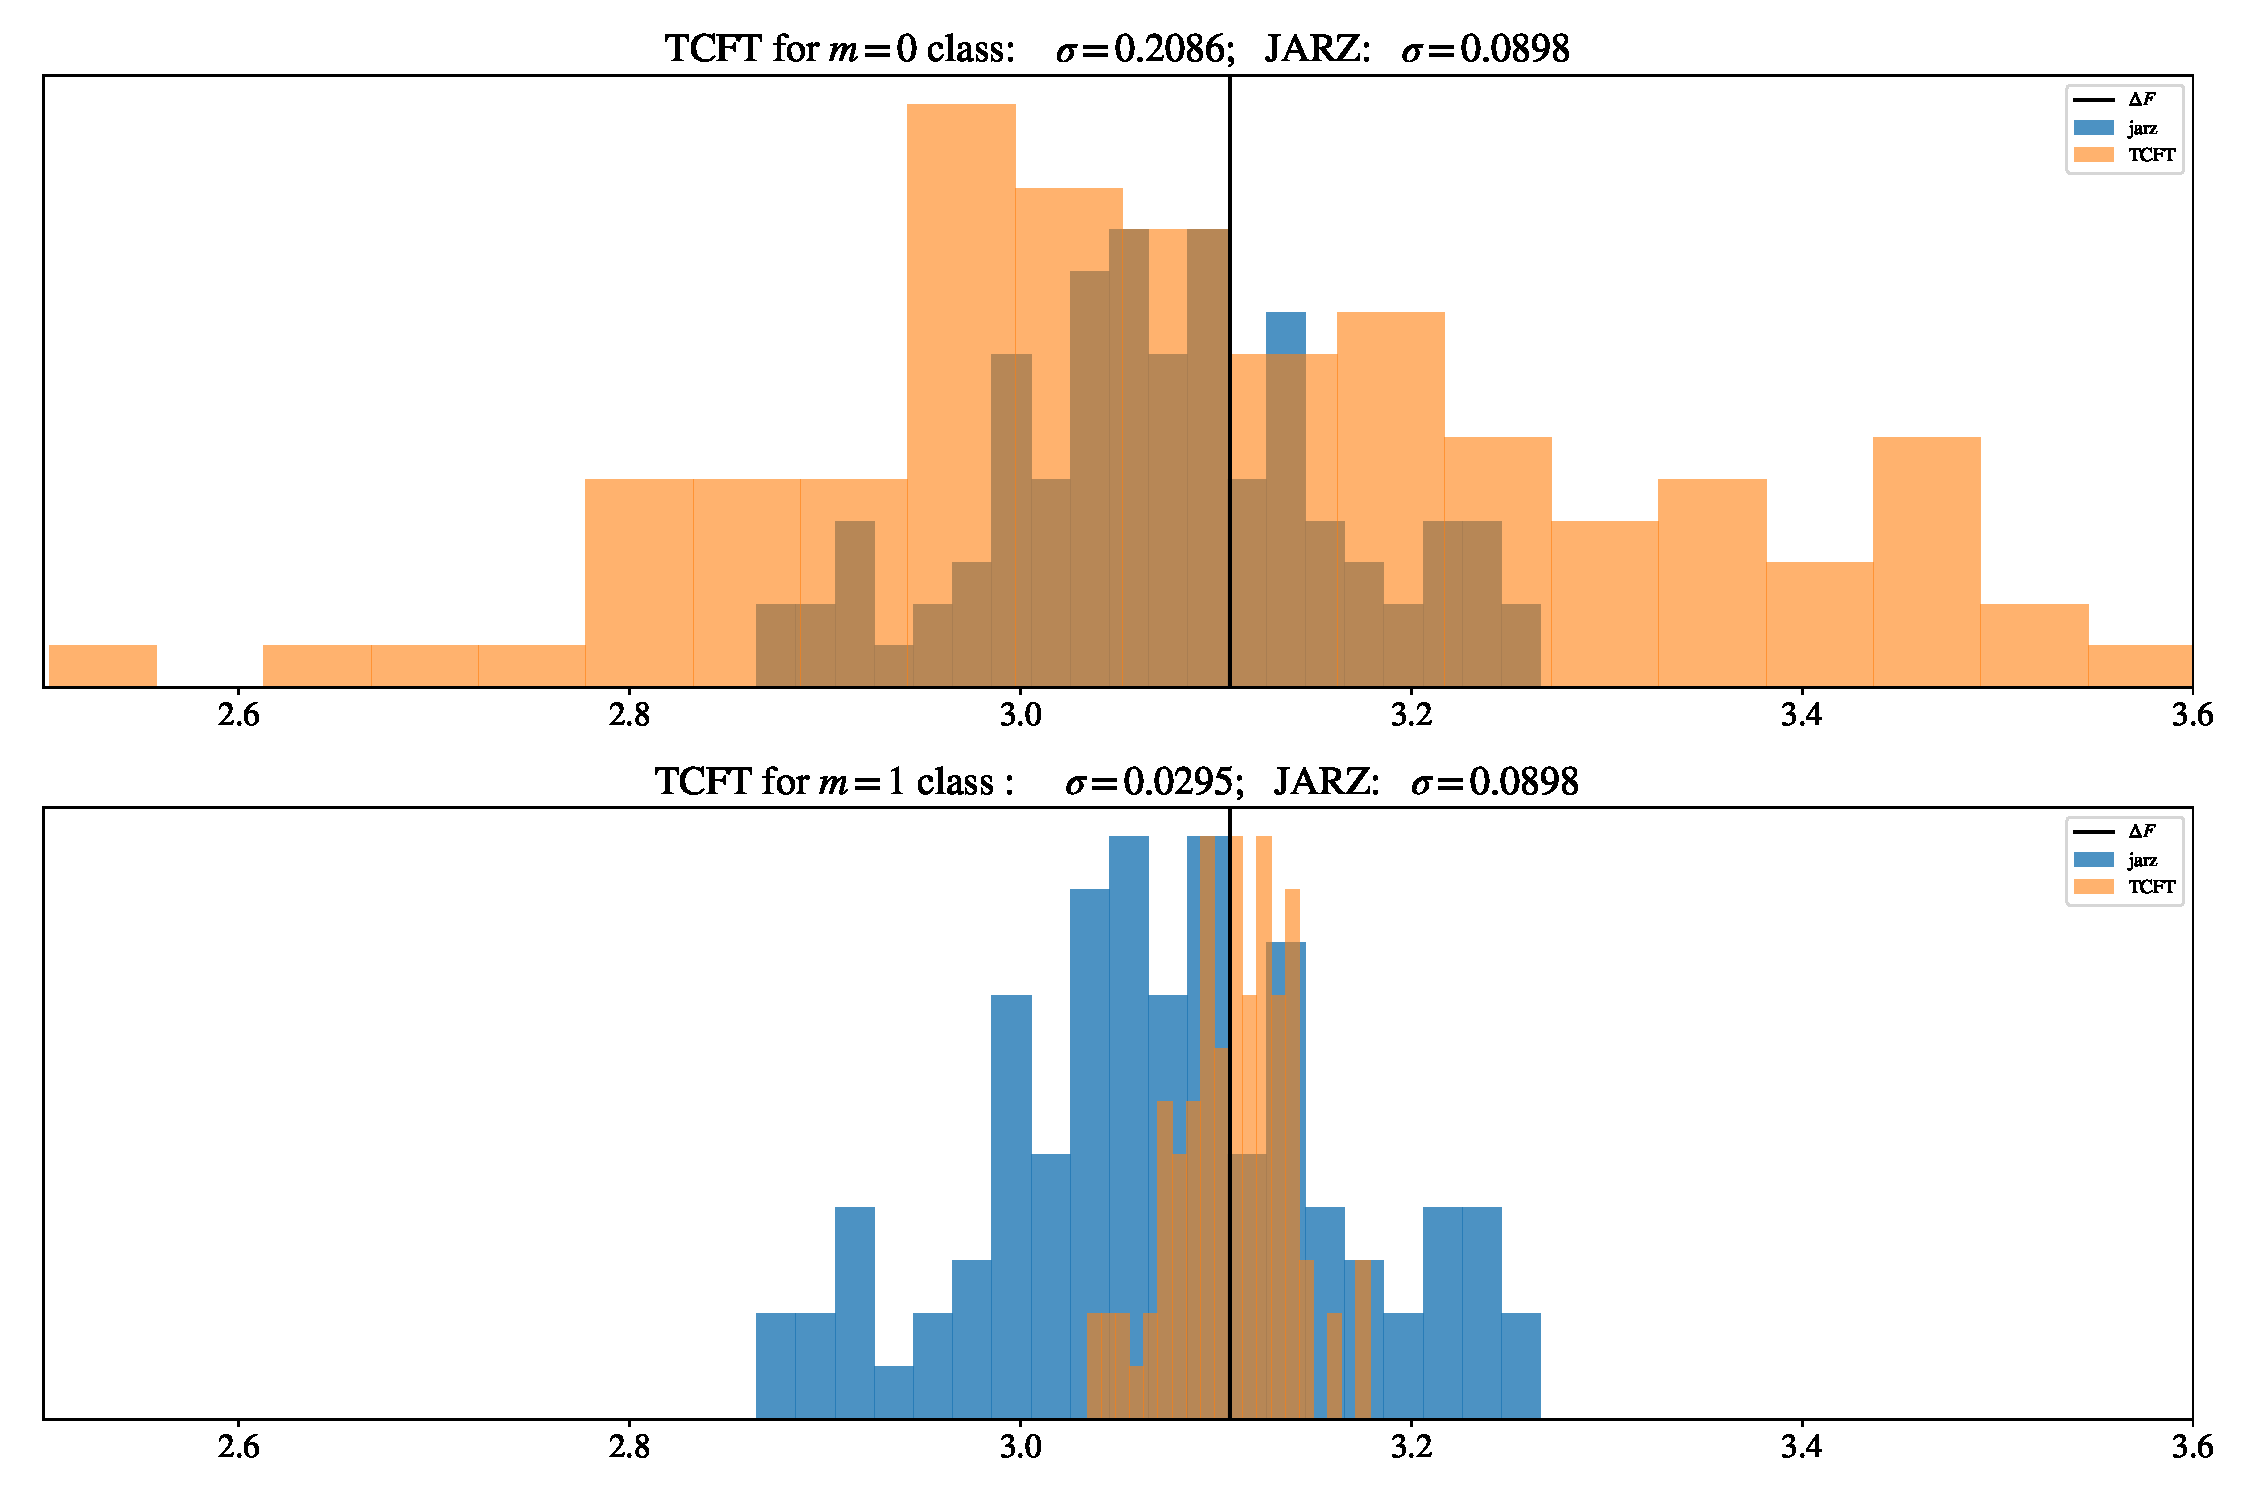
\includegraphics[width=.8\columnwidth, trim=0 0 0 0, clip]{ErrorCorrection.pdf}
\caption{Detailed study of two classes from figure \ref{fig:VarScaling}, (top) the class that always stays in the left well $0$ and (bottom) the class that always stays in the right well $1$. For each plot, 1000 trajectories were sampled 100 different times from a pool of 500,000 trajectories and the resulting estimate of the free energy was plotted using (blue) the JE and all trajectories and (orange) the TCFT and just the trajectories that belonged to the class in question.
}
\label{fig:ErrorCorrection}
\end{figure}

The analysis above is quite informative, but knowing which trajectory classes need the least statistics to be accurate does not on its own translate to a better experiment. For example, it might not be possible to select whichever class of trajectories is best. Instead, a more typical setup might be that a measurement device itself measures only a particular trajectory class which is not controlled by an experimenter so much as an inherent bias of the machine. For example, perhaps work values that fall under a certain threshold cannot be measured well because the measurement instrument is not sensitive to a work value that s much less than $\kB T$. Or, large energy fluctuations escape the detector and thus are ignored. These types of measurement shortcomings can cause additional bias uncertainty in the free energy estimate. From this perspective, the TCFT provides an invaluable tool take charge of these measurement errors-- reversing the effect of missing some trajectories. The question is slightly different here, so the experiment will also differ slightly. Instead of focusing on the scaling behavior of TCFT estimates across different classes and sample sizes, the focus will be on the TCFT as a correction to JE in the presence of a biased measurement device.

\begin{figure}
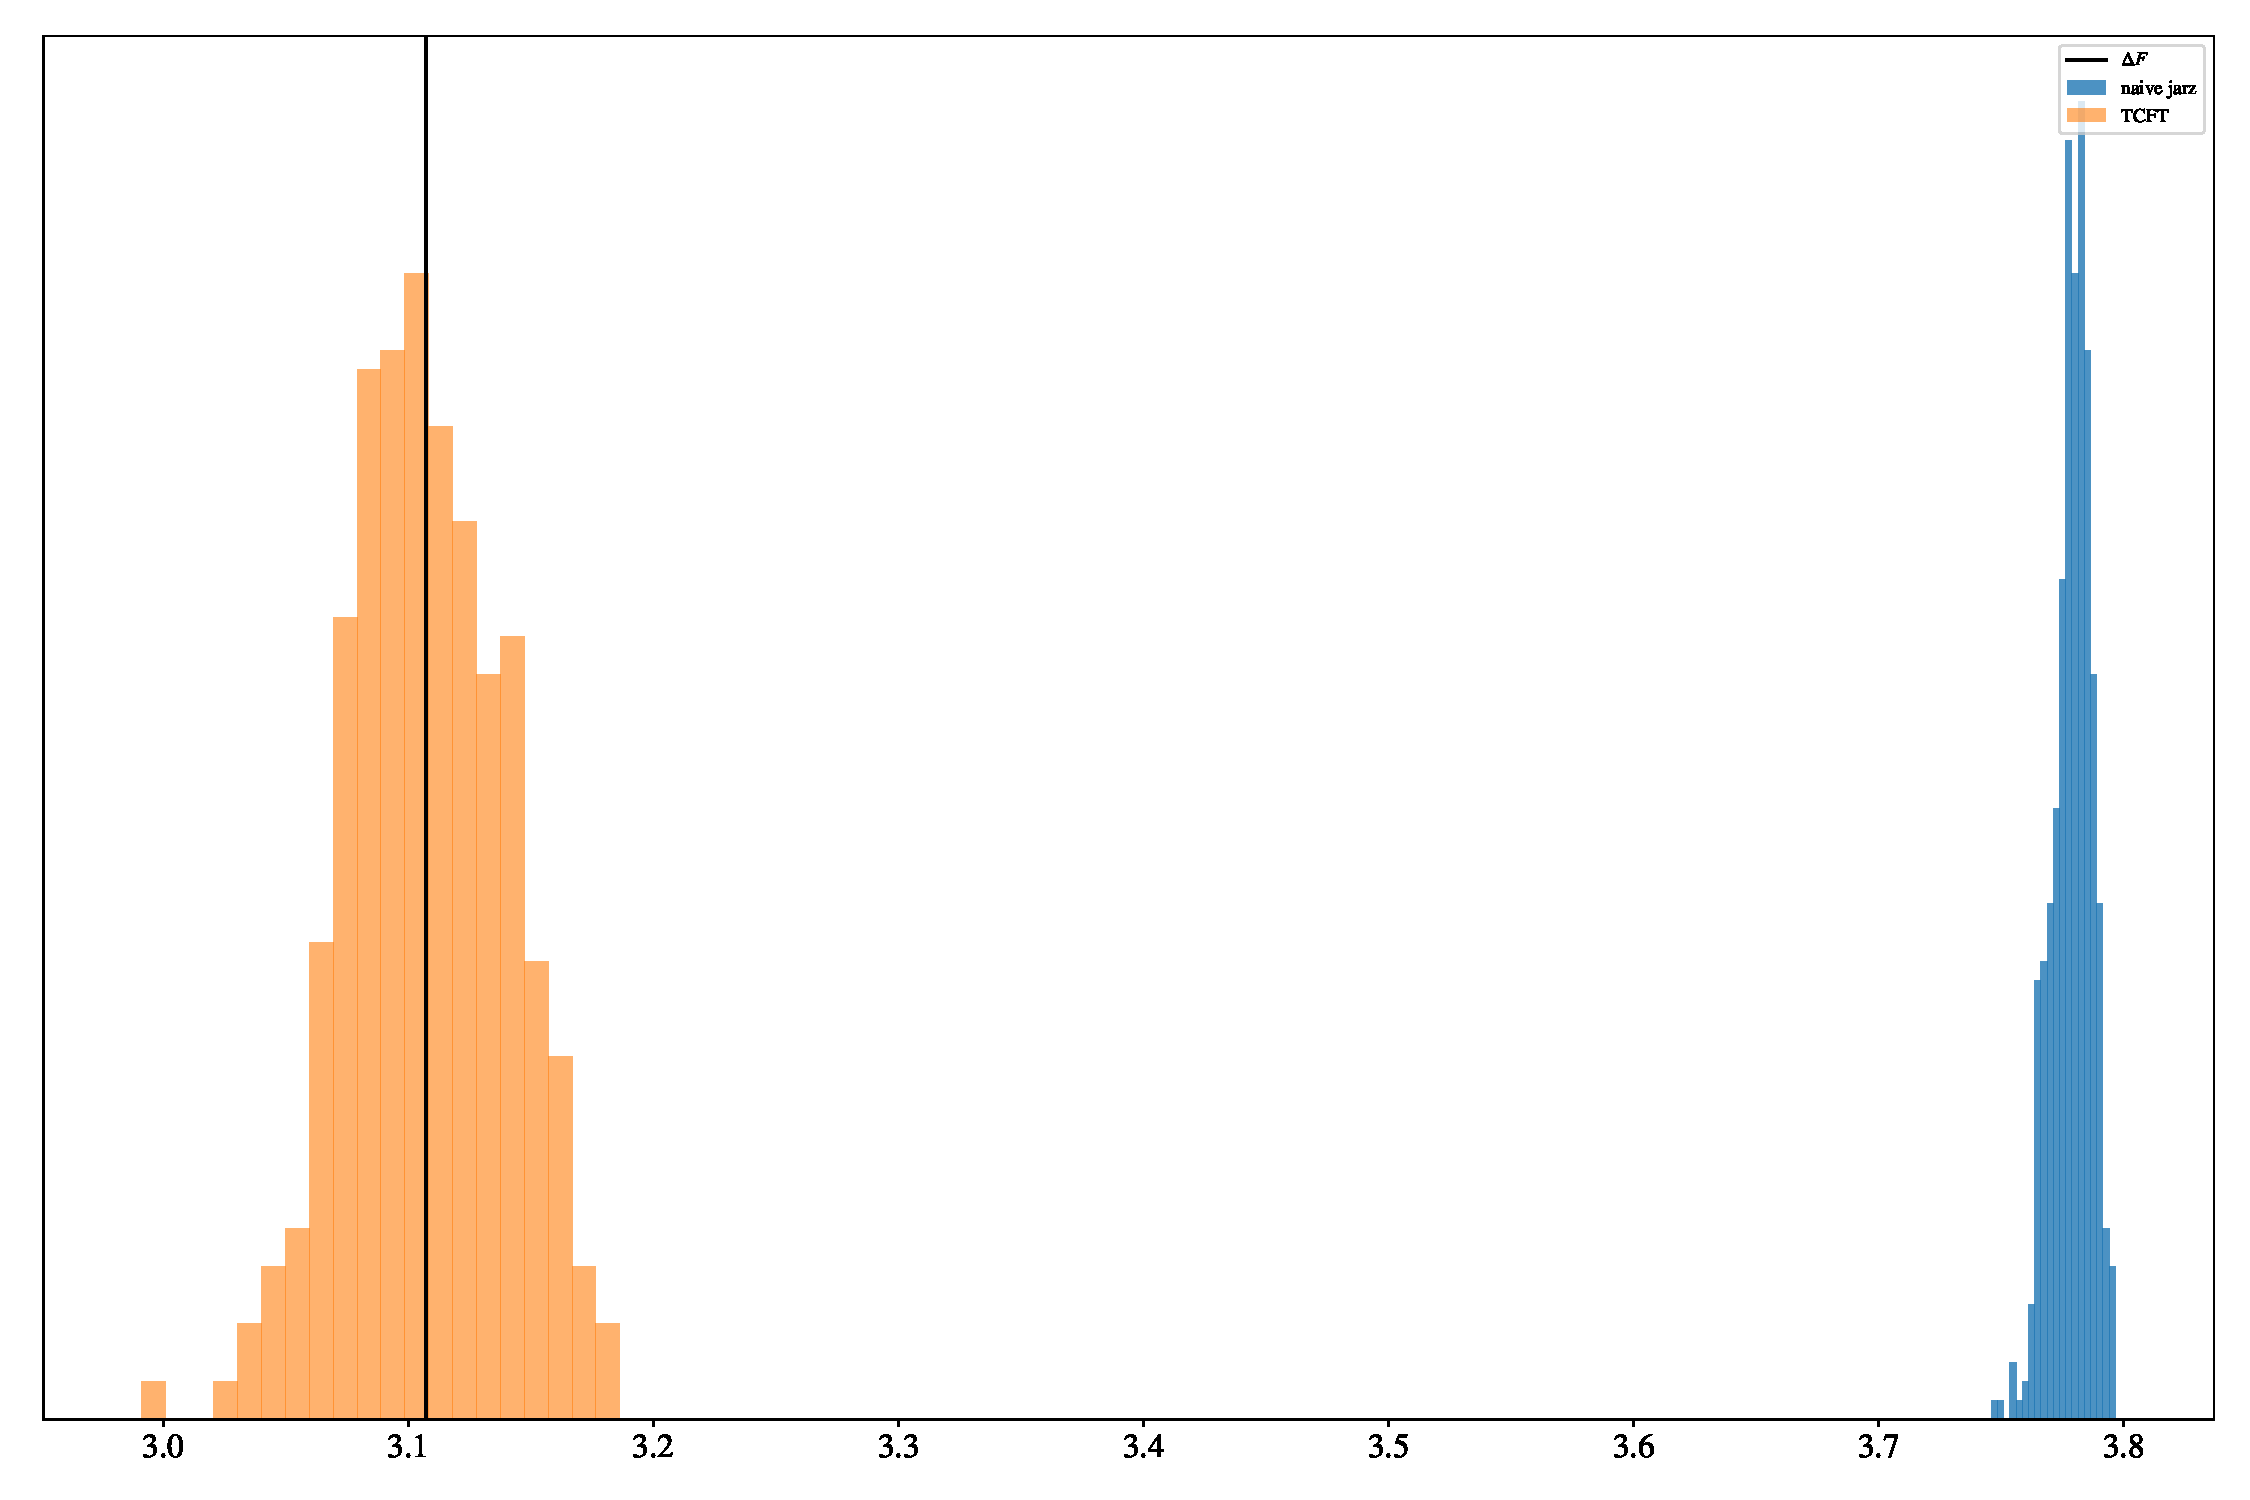
\includegraphics[width=.8\columnwidth, trim=0 0 0 0, clip]{BiasCorrection.pdf}
\centering
\caption{A histogram of taking 100 samples of 1000 trajectories each from a pool of 500,000 trajectories. In each case, a `naive Jarzynski' estimate was performed by throwing away the trials that did not fit in the class $0$, and then using the JE to estimate the free energy. The `TCFT' estimate was made by simulating the reverse trajectory and estimating the probability of the $0$ class.
}
\label{fig:BiasCorrection}
\end{figure}

 A first example will be the following: suppose the measurement device ignored every trajectory in the forward process that ever occupied the $0$ state. In this case, the experiment is still able to measure about $98\%$ of all trials-- and so it still might seem reasonable that it wont bias the free energy estimate too much. However, knowing that even rare events can dominate the free energy estimate, this might not be the case. Ignoring the TCFT, an experiment might use the faulty data-- knowing that a bias was inherent in the machine but unable to account for it. However, in this case the class that is missed by the machine is symmetric with respect to $C^\dagger$ conjugation, so if the probability of failing to measure a trajectory in the reverse process is estimated-- the TCFT can be used to completely correct the shortcomings of the machine. Figure \ref{fig:BiasCorrection} displays this by showing two different distributions. In one, the impoverished data is used to apply the JE to find the free energy and in the other and estimate of a measurement failure in the reserve process is estimated as well (by simulation) and then the TCFT is used. It is immediately obvious that the missing $2\%$ of trajectories provides an enormous bias to the result, but that the TCFT is able to reverse the bias even with relatively few trials. The additional error in the TCFT corrected distribution comes from having to estimate both $P(C)$ and $R(C)$.

\subsection{Metastable Free Energy}
Returning to the idea of  local free energies, and metastable processes. Imagine that we have a system that has a number of metastable regions with local equilibration timescales $\tau^m$ that are all much shorter than the global equilibration timescale $\tau_0$. Assume that we want to find out the local free energies associated with each region, or more specifically, the $\Delta F_{ij}$ from equation \ref{LocalFreeEnergy} between two regions, and are able at any point in time to observe which metastable region a particle is in. By initializing a particle into one of these regions, and tracking the trajectory it takes over some long time period $\tau_\infty >> \tau_0$, we should be able to model the inter-region dynamics as a continuous time markov chain and estimate the transition probabilities between regions. This will give us the equilibrium distribution which can be used to find $\frac{Z_i}{Z_j}$, and thus $\Delta F_{ij}$. However, note that the time it would take to do this is governed by the global equilibration timescale-- which might be very large. \tbf{tbd: statistical analysis of how long we would need to wait in order to nicely estimate the free energy between two wells with this kind of passive process as a function of the barrier energy, then can compare this to the TCFT application}


If, on top of being able to track the coarse grained region, we also have the ability to control the system and measure the work done on it by this control, then the TCFT provides us with a faster avenue to obtain the local free energy landscape through equation \ref{LocalFreeEnergy}
\begin{align}
\beta \Delta F_{ij} =  -\ln \avg{e^{-\beta W }}_{ij}- \ln \frac{P(C_{ij})}{R(C_{ij})} - \ln \frac{u^j}{w^i} 
~. 
\end{align}

\begin{figure}
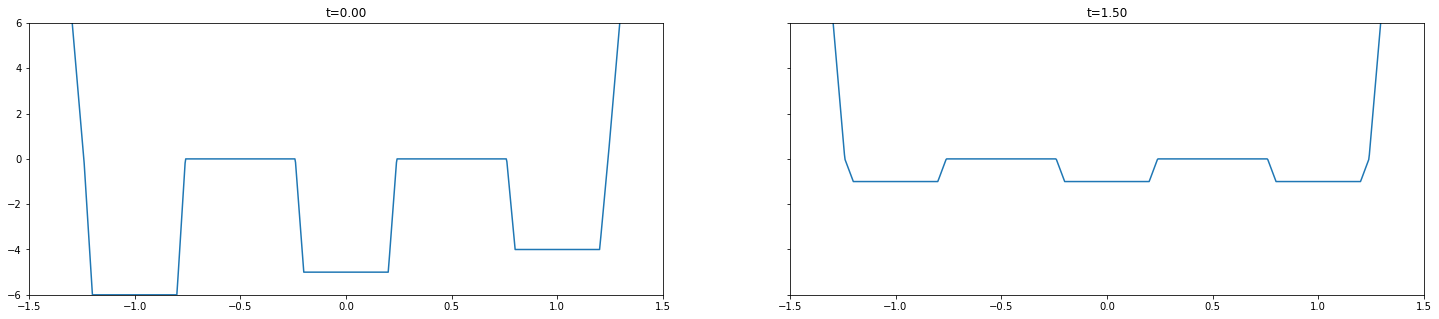
\includegraphics[width=\columnwidth, trim=0 0 0 0, clip]{square_trip.png}
\centering
\caption{Ignore the numbers here, this should just be labeled with variables. Also assume the walls are vertical rather than just steep}
\label{fig:SquareTrip}
\end{figure}

Let's set $\beta=1$, to consider a simple example: a system exposed to potential energy profile that looks like the left panel of fig. \ref{fig:SquareTrip}. We have three metastable regions $L,C,R$ with the same width $D$, and associated potential energies $-E_L, -E_C, -E_R$ with barriers between them at $E=0$ and widths $D_B$. Transitions between these regions will be much slower than transitions within the regions because of the energy barriers that separate them are larger than $k_B T$ (\tbf{maybe add in the analytic result of transition times as a function of barrier height}). Assume that we begin in some metastable distribution $w_0 = (w_L, w_C, w_R, 0, 0)$ (the two trailing zeros correspond to a zero probability of starting on either barrier). We then perturb the system in such a way that facilitates transitions between the regions, say by changing the energy profile to the right panel of the fig. \ref{fig:SquareTrip} where the metastable regions have been made degenerate and had their barrier energies significantly reduced to $-E_0$. This potential is held for a long enough time that the particles equilibrate to this new potential, and then the perturbation is reversed, and since the local equilibrium in each well is uniform-- we are already in a metastable distribution immediately after the perturbation is reversed.

Now, in this simple case because all regions have a constant potential energy we have $Z_m = D_m e^{E_m}$, so once the particles have equilibrated to the perturbed drive the metastable weights become the equilibrium weights $w_1 = ( w_1, w_1, w_1, w_B, w_B)$ with $w_1 = De^{E_0} (3*De^{E_0}+2D_B)^{-1}$ and $w_B = D_B (3*De^{E_0}+2D_B)^{-1}$. Now, let's use as our trajectory class all those trajectories that started in the left well, and ended in the center well right before the perturbation was reserved. Because every member of this class begins and ends in the same metastable region, we can use the relation above. Notably, every trajectory in this class has the same work value of $E_C - E_L$ which means we have

\begin{align}
\log \frac{Z_C}{Z_L} &=  E_C - E_L - \ln \frac{P(C_{})}{R(C_{ij})} - \ln \frac{u^j}{w^i} \\
E_C-E_L &=  E_C - E_L - \ln \frac{P(C_{ij})}{R(C_{ij})} - \ln \frac{u^j}{w^i}
~. 
\end{align}
Telling us that the final two terms must work out to be zero. And, upon inspection-- we find that they are. $P(C_{LC}) = w_L \cdot w_1$ (we can do this because the particle was allowed to equilibrate during the perturbation, so there is no correlation between the initial and final state). In this case, because the perturbation was reverse-- the protocol is time symmetric, so $P$ and $R$ are the same protocol. Thus, $R(C_{LC}) = w_L \cdot w_L$. Putting this all together, the full sum gives
\begin{align}
- \ln \frac{w_L w_1}{w_L^2}  - \ln \frac{w_L}{w_1} = 0
~. 
\end{align}

\begin{figure}
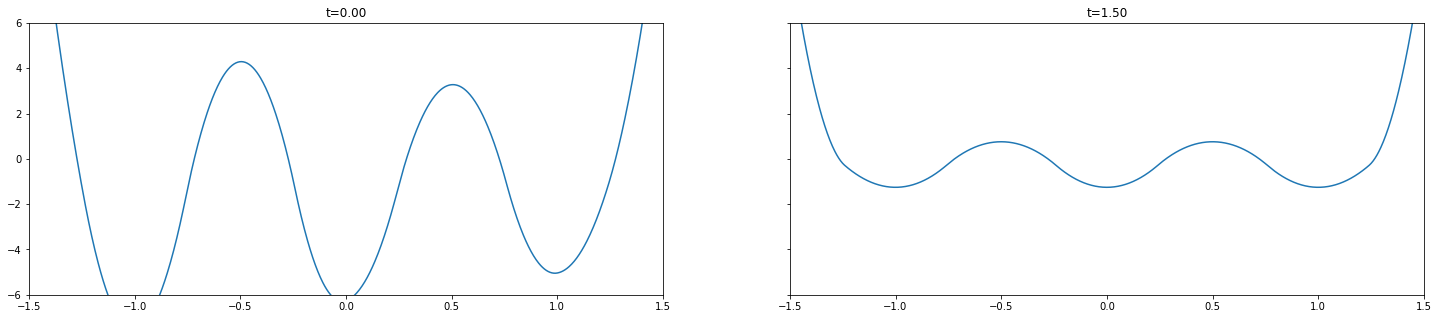
\includegraphics[width=\columnwidth, trim=0 0 0 0, clip]{quad_trip.png}
\centering
\caption{(left) the Unperturbed and (right) perturbed potentials for the simulation}
\label{fig:QuadTrip}
\end{figure}
While this example is quite simplified, the remarkable fact is that the equality holds no matter how far out of equilibrium the perturbation takes the system and wether or not we know anything about the nature of the perturbation or the local curvature within each metastable region. (\tbf{a first oder correction to this would be to allow particles to fall off of the barriers into the wells after the perturbation is reversed, this should also be analytically calculable and might be more compelling?}). This remarkable fact can be demonstrated in simulation, by using a smooth potential energy profiles like those show in in fig \ref{fig:QuadTrip}. Using overdamped Langevin dynamics, we can take advantage of the much faster rate at which the particles explore the perturbed potential to come up with estimates of $\Delta F_{ij}$ for the unperturbed potential.

Using the same type of protocol as described for the constant energy wells, we can estimate $\Delta F_{ij}$ with decent accuracy and relatively few trials. See fig \ref{fig:MetastableSims}
\begin{figure}
\centering
\subfloat[]{\includegraphics[width=.5\columnwidth, trim=0 0 0 0, clip]{trajectories.png}}
\subfloat[]{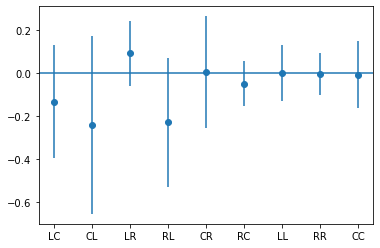
\includegraphics[width=.5\columnwidth, trim=0 0 0 0, clip]{Fij_estimate.png}}
\caption{(a) 200 sample trajectories chosen from a uniform distribution over all three wells. One can see explicitly how the perturbed potential allows for the particles to explore the state space much quicker than keeping the unperturbed potential. (b) Each possible trajectory class, plotted against the difference between the estimated $\Delta F_{ij}$ using the simulation statistics and the actual $\Delta F_{ij}$ calculated numerically from the exact potential energy profile.}
\label{fig:MetastableSims}
\end{figure}

\end{document}


%% TEMPLATES FOR REFERENCE%%%%%%
%%%%%%%%%%%%%%%%%%%%%%%%%

% \begin{figure}[H]
 %\centering
  % \subfloat[]{\includegraphics[width=.8\textwidth]{3figcount1.png}}\\
 %\subfloat[]{\includegraphics[width=.8\textwidth]{3figcount2.png}}
%\end{figure}


%\begin{figure}[H]
%\centering
%\includegraphics[scale=1]{2fig1.pdf}
%\caption{pn junction before (left) and after (right) coming into contact and achieving equilibrium. p type is on the left and n type is on the right}
%\end{figure}

%\usepackage{pdfpages}
%\includepdf[pages={1-7}]{HW4.pdf}


%\begin{enumerate}[align=parleft,labelsep=26pt]
%\item[a]
%\end{enumerate}


